

%% CAP High School Prize Examination
%%----------------------------------------


%% this section contains 40 problems


%% CAP Exam 2015
%%----------------------------------------
\element{cap}{ %% CAP-C3
\begin{question}{CAP-A-2015-q10}
    A constant amount of ideal gas, at the temperature $T_0$,
        undergoes a process that changes its pressure from $P_0$ to $2P_0$.
    Then its volume is increased from $V_0$ to $3V_0$ at a constant pressure,
        as shown on the $PV$ diagram:
    \begin{center}
    \begin{tikzpicture}
        \begin{axis}[
            axis y line=left, 
            axis x line=bottom, 
            axis line style={->},
            xlabel={volume},
            xtick={0,1,2,3},
            xticklabels={0,$V_0$,$2V_0$,$3V_0$},
            ylabel={pressure},
            ytick={0,1,2},
            yticklabels={0,$p_0$,$2p_0$},
            xmin=0,xmax=3.5,
            ymin=0,ymax=2.5,
            width=0.8\columnwidth,
            height=0.5\columnwidth,
        ]
        \addplot[line width=1pt,mark=*] plot coordinates { (1,1) (1,2) (3,2) };
        \node[anchor=west] at (axis cs:1,1) {1};
        \node[anchor=south] at (axis cs:1,2) {2};
        \node[anchor=south] at (axis cs:3,2) {3};
        \draw[dashed] (axis cs:1,0) -- (axis cs:1,1);
        \draw[dashed] (axis cs:0,1) -- (axis cs:1,1);
        \draw[dashed] (axis cs:0,2) -- (axis cs:1,2);
        \draw[dashed] (axis cs:3,0) -- (axis cs:3,2);
        \end{axis}
    \end{tikzpicture}
    \end{center}
    Which of the $PT$ diagrams below correctly reflects these processes:
    \begin{choices}
        \AMCboxDimensions{down=-4.5em}
        \wrongchoice{
            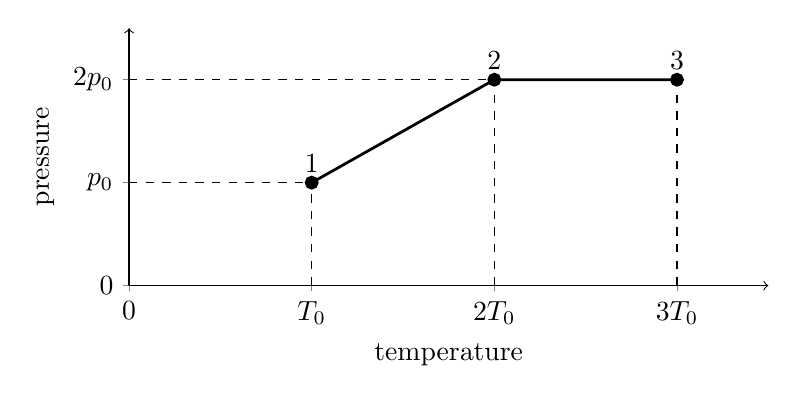
\begin{tikzpicture}
                \begin{axis}[
                    clip=false,
                    axis y line=left, 
                    axis x line=bottom, 
                    axis line style={->},
                    xlabel={temperature},
                    xtick={0,1,2,3},
                    xticklabels={0,$T_0$,$2T_0$,$3T_0$},
                    ylabel={pressure},
                    ytick={0,1,2},
                    yticklabels={0,$p_0$,$2p_0$},
                    xmin=0,xmax=3.5,
                    ymin=0,ymax=2.5,
                    width=0.8\columnwidth,
                    height=0.4\columnwidth,
                ]
                \addplot[line width=1pt,mark=*] plot coordinates { (1,1) (2,2) (3,2) };
                \node[anchor=south] at (axis cs:1,1) {1};
                \node[anchor=south] at (axis cs:2,2) {2};
                \node[anchor=south] at (axis cs:3,2) {3};
                \draw[dashed] (axis cs:0,1) -- (axis cs:1,1);
                \draw[dashed] (axis cs:0,2) -- (axis cs:2,2);
                \draw[dashed] (axis cs:1,0) -- (axis cs:1,1);
                \draw[dashed] (axis cs:2,0) -- (axis cs:2,2);
                \draw[dashed] (axis cs:3,0) -- (axis cs:3,2);
                \end{axis}
            \end{tikzpicture}
        }
        %% ANS is B
        \correctchoice{
            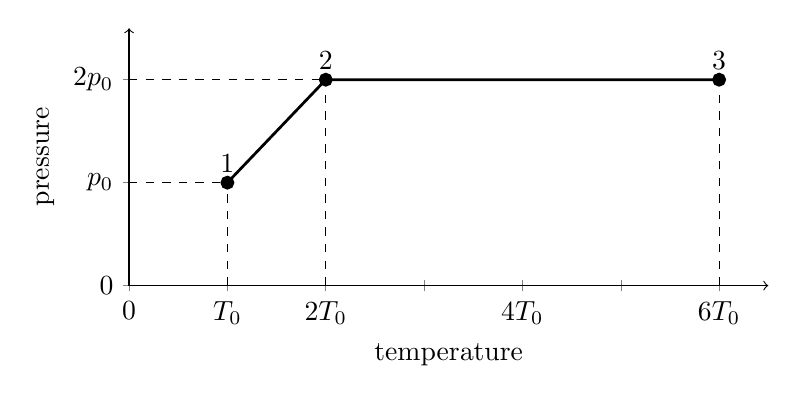
\begin{tikzpicture}
                \begin{axis}[
                    clip=false,
                    axis y line=left, 
                    axis x line=bottom, 
                    axis line style={->},
                    xlabel={temperature},
                    xtick={0,1,2,3,4,5,6},
                    xticklabels={0,$T_0$,$2T_0$,,$4T_0$,,$6T_0$},
                    ylabel={pressure},
                    ytick={0,1,2},
                    yticklabels={0,$p_0$,$2p_0$},
                    xmin=0,xmax=6.5,
                    ymin=0,ymax=2.5,
                    width=0.8\columnwidth,
                    height=0.4\columnwidth,
                ]
                \addplot[line width=1pt,mark=*] plot coordinates { (1,1) (2,2) (6,2) };
                \node[anchor=south] at (axis cs:1,1) {1};
                \node[anchor=south] at (axis cs:2,2) {2};
                \node[anchor=south] at (axis cs:6,2) {3};
                \draw[dashed] (axis cs:0,1) -- (axis cs:1,1);
                \draw[dashed] (axis cs:0,2) -- (axis cs:2,2);
                \draw[dashed] (axis cs:1,0) -- (axis cs:1,1);
                \draw[dashed] (axis cs:2,0) -- (axis cs:2,2);
                \draw[dashed] (axis cs:6,0) -- (axis cs:6,2);
                \end{axis}
            \end{tikzpicture}
        }
        \wrongchoice{
            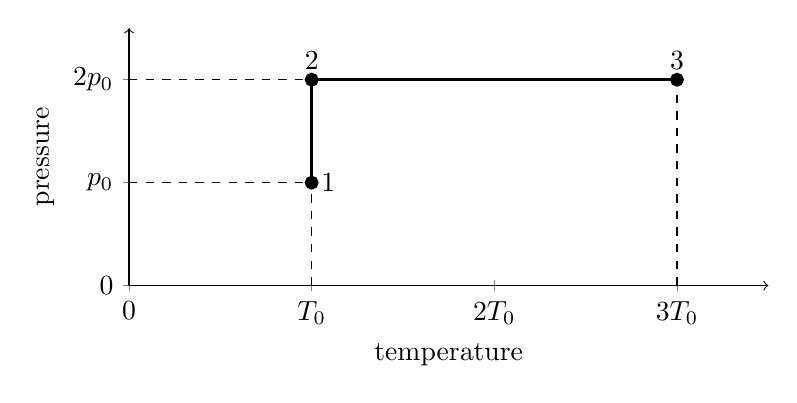
\begin{tikzpicture}
                \begin{axis}[
                    clip=false,
                    axis y line=left, 
                    axis x line=bottom, 
                    axis line style={->},
                    xlabel={temperature},
                    xtick={0,1,2,3},
                    xticklabels={0,$T_0$,$2T_0$,$3T_0$},
                    ylabel={pressure},
                    ytick={0,1,2},
                    yticklabels={0,$p_0$,$2p_0$},
                    xmin=0,xmax=3.5,
                    ymin=0,ymax=2.5,
                    width=0.8\columnwidth,
                    height=0.4\columnwidth,
                ]
                \addplot[line width=1pt,mark=*] plot coordinates { (1,1) (1,2) (3,2) };
                \node[anchor=west] at (axis cs:1,1) {1};
                \node[anchor=south] at (axis cs:1,2) {2};
                \node[anchor=south] at (axis cs:3,2) {3};
                \draw[dashed] (axis cs:0,1) -- (axis cs:1,1);
                \draw[dashed] (axis cs:0,2) -- (axis cs:1,2);
                \draw[dashed] (axis cs:1,0) -- (axis cs:1,1);
                \draw[dashed] (axis cs:3,0) -- (axis cs:3,2);
                \end{axis}
            \end{tikzpicture}
        }
        \wrongchoice{
            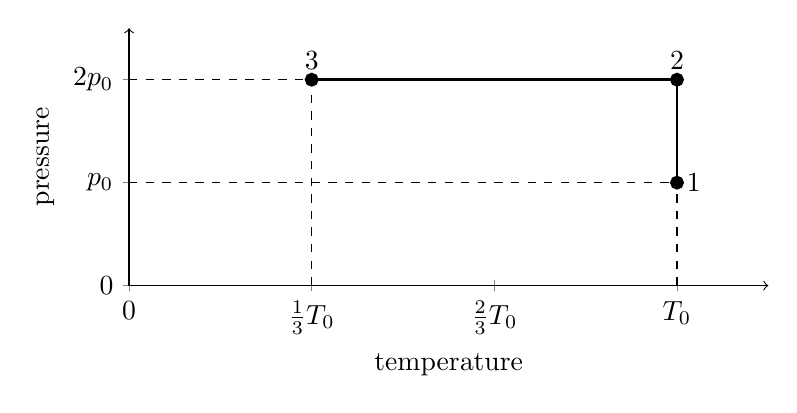
\begin{tikzpicture}
                \begin{axis}[
                    clip=false,
                    axis y line=left, 
                    axis x line=bottom, 
                    axis line style={->},
                    xlabel={temperature},
                    xtick={0,1,2,3},
                    xticklabels={0,$\frac{1}{3}T_0$,$\frac{2}{3}T_0$,$T_0$},
                    ylabel={pressure},
                    ytick={0,1,2},
                    yticklabels={0,$p_0$,$2p_0$},
                    xmin=0,xmax=3.5,
                    ymin=0,ymax=2.5,
                    width=0.8\columnwidth,
                    height=0.4\columnwidth,
                ]
                \addplot[line width=1pt,mark=*] plot coordinates { (1,2) (3,2) (3,1) };
                \node[anchor=west] at (axis cs:3,1) {1};
                \node[anchor=south] at (axis cs:3,2) {2};
                \node[anchor=south] at (axis cs:1,2) {3};
                \draw[dashed] (axis cs:0,1) -- (axis cs:3,1);
                \draw[dashed] (axis cs:0,2) -- (axis cs:1,2);
                \draw[dashed] (axis cs:1,0) -- (axis cs:1,2);
                \draw[dashed] (axis cs:3,0) -- (axis cs:3,1);
                \end{axis}
            \end{tikzpicture}
        }
    \end{choices}
\end{question}
}


\endinput


